%%
%% This is file `sample-acmtog.tex',
%% generated with the docstrip utility.
%%
%% The original source files were:
%%
%% samples.dtx  (with options: `all,journal,bibtex,acmtog')
%% 
%% IMPORTANT NOTICE:
%% 
%% For the copyright see the source file.
%% 
%% Any modified versions of this file must be renamed
%% with new filenames distinct from sample-acmtog.tex.
%% 
%% For distribution of the original source see the terms
%% for copying and modification in the file samples.dtx.
%% 
%% This generated file may be distributed as long as the
%% original source files, as listed above, are part of the
%% same distribution. (The sources need not necessarily be
%% in the same archive or directory.)
%%
%%
%% Commands for TeXCount
%TC:macro \cite [option:text,text]
%TC:macro \citep [option:text,text]
%TC:macro \citet [option:text,text]
%TC:envir table 0 1
%TC:envir table* 0 1
%TC:envir tabular [ignore] word
%TC:envir displaymath 0 word
%TC:envir math 0 word
%TC:envir comment 0 0
%%
%% The first command in your LaTeX source must be the \documentclass
%% command.
%%
%% For submission and review of your manuscript please change the
%% command to \documentclass[manuscript, screen, review]{acmart}.
%%
%% When submitting camera ready or to TAPS, please change the command
%% to \documentclass[sigconf]{acmart} or whichever template is required
%% for your publication.
%%
%%
\documentclass[acmtog]{acmart}
%%
%% \BibTeX command to typeset BibTeX logo in the docs
\AtBeginDocument{%
  \providecommand\BibTeX{{%
    Bib\TeX}}}

%% Rights management information.  This information is sent to you
%% when you complete the rights form.  These commands have SAMPLE
%% values in them; it is your responsibility as an author to replace
%% the commands and values with those provided to you when you
%% complete the rights form.
\setcopyright{acmlicensed}
\copyrightyear{2025}
\acmYear{2025}
\acmDOI{XXXXXXX.XXXXXXX}

%%
%% Submission ID.
%% Use this when submitting an article to a sponsored event. You'll
%% receive a unique submission ID from the organizers
%% of the event, and this ID should be used as the parameter to this command.
%%\acmSubmissionID{123-A56-BU3}

%%
%% For managing citations, it is recommended to use bibliography
%% files in BibTeX format.
%%
%% You can then either use BibTeX with the ACM-Reference-Format style,
%% or BibLaTeX with the acmnumeric or acmauthoryear sytles, that include
%% support for advanced citation of software artefact from the
%% biblatex-software package, also separately available on CTAN.
%%
%% Look at the sample-*-biblatex.tex files for templates showcasing
%% the biblatex styles.
%%

%%
%% The majority of ACM publications use numbered citations and
%% references.  The command \citestyle{authoryear} switches to the
%% "author year" style.
%%
%% If you are preparing content for an event
%% sponsored by ACM SIGGRAPH, you must use the "author year" style of
%% citations and references.
\citestyle{acmauthoryear}


%%
%% end of the preamble, start of the body of the document source.
\begin{document}

%%
%% The "title" command has an optional parameter,
%% allowing the author to define a "short title" to be used in page headers.
\title{Analyzing 5G Network Vulnerabilities with a Forward Look into 6G Security}

%%
%% The "author" command and its associated commands are used to define
%% the authors and their affiliations.
%% Of note is the shared affiliation of the first two authors, and the
%% "authornote" and "authornotemark" commands
%% used to denote shared contribution to the research.

\author{Josue Lopez}
\affiliation{%
  \institution{California Polytechnic State University, San Luis Obispo}
  \city{San Luis Obispo}
  \country{USA}}
\email{jlope424@calpoly.edu}

\author{Noah Giboney}
\affiliation{%
  \institution{California Polytechnic State University, San Luis Obispo}
  \city{San Luis Obisp}
  \country{USA}
}
\email{ngiboney@calpoly.edu}

\author{Peter Kallos}
\affiliation{%
 \institution{California Polytechnic State University, San Luis Obispo}
 \city{San Luis Obisp}
 \country{USA}}
 \email{pkallos@calpoly.edu}


%%
%% By default, the full list of authors will be used in the page
%% headers. Often, this list is too long, and will overlap
%% other information printed in the page headers. This command allows
%% the author to define a more concise list
%% of authors' names for this purpose.
\renewcommand{\shortauthors}{Lopez et al.}

%%
%% The abstract is a short summary of the work to be presented in the
%% article.
\begin{abstract}
  The rapid evolution of wireless communication technologies from 5G to 6G presents both
  unprecedented opportunities and significant security challenges. While 5G enables enhanced
  connectivity, high data rates and support for emerging applications such as autonomous vehicles
  and massive IoT, it also introduces a broader attack surface and increased vulnerability across 
  the network stack. As the research community prepares for the rollout of 6G, new technological 
  and architectural shifts, such as AI-native infrastructure, visible light communication and
  sub-terahertz spectrum use, pose security concerns distinct from those in 5G. This survery paper
  analyzes existing vulnerabilities in 5G networks and investigates how proposed technologies for 6G
  may both mitigate and exacerbate security risks. Our goal is to provide a holistic understanding of
  the wireless network security landscape and to assess how well the 6G paradigm addresses the limitations of its predecessor.
\end{abstract}


%%
%% Keywords. The author(s) should pick words that accurately describe
%% the work being presented. Separate the keywords with commas.
\keywords{5G Security, 6G Networks, Network Vulnerabilities, Wireless  Communication, Cybersecurity, Mobile Network Security}

%%
%% This command processes the author and affiliation and title
%% information and builds the first part of the formatted document.
\maketitle

\section{Introduction}

\section{Review of 5G Security: Advantages and Vulnerabilities}
The progression of wireless communication standards and next generation data systems tend to provide faster data speeds, lower latency, and greater connectivity among devices. 5G has introduced all these improvements in performance, enabling services such as autonomous vehicles and mobile broadband communications to operate more efficiently and at a much larger scale. With these new capabilities, however, comes a broader and more complex attack surface for malicious actors to exploit. This section reviews three foundational papers \cite{ref3}, \cite{ref6}, \cite{ref7} to showcase 5G's benefits and the security challenges they create.

\subsection{Advantages of 5G Technology}
5G networks deliver enhanced mobile broadband (eMBB), ultra-reliable low-latency communications (uRLLC), and massive machine-type communications (mMTC) \cite{ref6}. These applications are the product of some of the core technologies used in 5G which include software-defined networking (SDN), network function virtualization (NFV), network slicing, and mobile edge computing (MEC). All of them come together to create networks that are efficient, flexible, and dynamic. 

\subsubsection{SDN Advantages} SDN is a network management approach that separates the control plane from the data plane to allow for the centralized control and programmability of network infrastructure. In SDN, a logically centralized controller manages network behavior through standardized protocols like OpenFlow to enable the configuration of network components \cite{ref3}. SDN enhances mobile networks by providing near real-time network control and efficient resource sharing \cite{ref6_1}. It provides an easy way to manage different kinds of hardware, backhaul technologies, and configuration interfaces to enable flexible network connectivity and service provisioning between edge-to-edge networks over various transport systems \cite{ref6_1}. SDN helps solve problems like IP address translation, control signaling overhead, and tunneling by dynamically adjusting traffic flows or tuning codec schemes for wireless links \cite{ref6_1}. Within mobile networks, SDN enables cross-layer coordination between the mobile and transport layers. This allows flow tables in switches and routers to be updated directly without the need to reroute traffic to new switches and routers. This eliminates the need for IP address translation and tunneling which is useful for user mobility in MEC setups \cite{ref6_1}. SDN is what allows 5G to be user-centric, flexible, scalable, achieve high capacity, and provide low latency \cite{ref6}.
\begin{figure}[h]
  \centering
  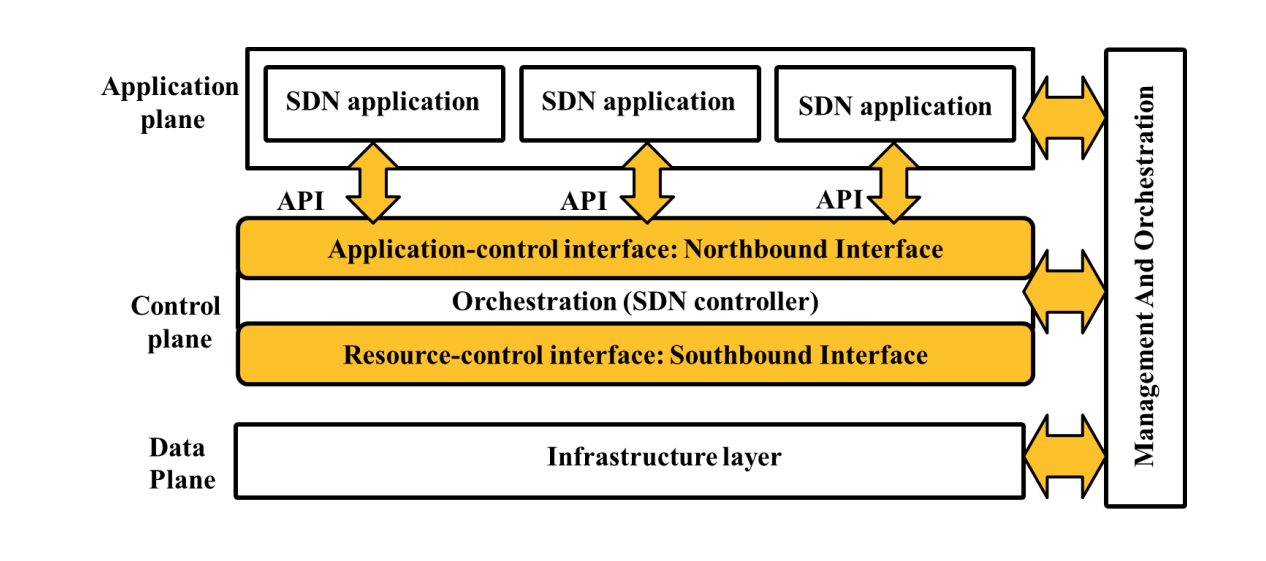
\includegraphics[width=\linewidth]{sdn.png}
  \caption{SDN layered architecture \cite{ref7_1}}
\end{figure}


\subsubsection{NFV Advantages} NFV enhances traditional network operations by virtualizing network services (e.g. routers, firewalls, load balancers) that were historically implemented on dedicated hardware. The software that provide this virtualization are known as virtual network functions (VNFs). Additionally, the NFV infrastructure (NFVI) encompasses hardware and software components like CPUs, storage, and virtualization layers. This provides the environment for VNF deployment. There's also NFV management and orchestration (NFV MANO) which manages the life cycle management of VNFs and the organization of physical and virtual resources within the NFVI \cite{ref6_1}. NFV MANO also handles fault management scenarios like replacing a virtual machine (VM) when it fails, and supports connectivity across MEC platforms deployed in different locations. This can be effective when integrated with SDN for service chaining (linking different network services like firewalls, load balancers, and routers in a specific order to handle network traffic) \cite{ref6_1}. NFV works closely with SDN, complementing it to provide flexibility, scalability, and low latency (but not high capacity) seen in 5G networks \cite{ref6}.
\begin{figure}[h]
  \centering
  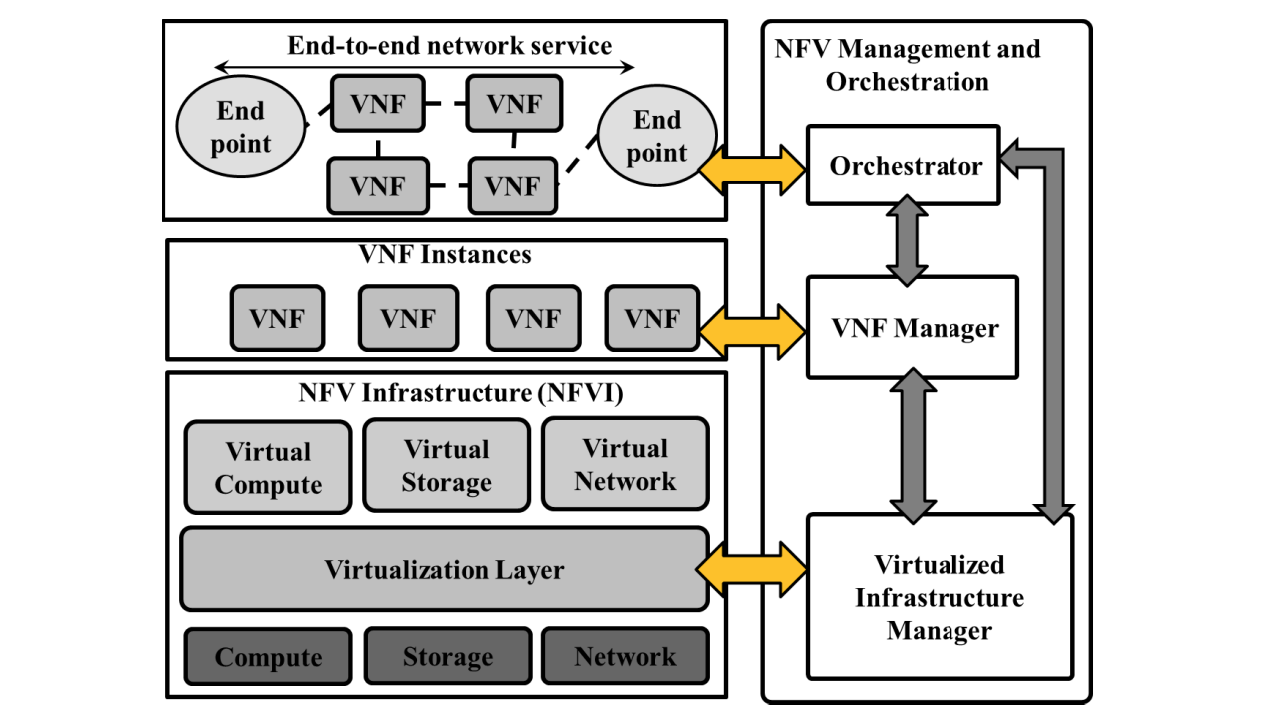
\includegraphics[width=\linewidth]{nfv.png}
  \caption{NFV high level architecture \cite{ref7_1}}
\end{figure}

\subsubsection{Network Slicing Advantages} Network slicing divides a single physical network into various smaller networks known as a network slice. These individual slices can be specialized for a specific type of service or application and can be made of both virtualized and non-virtualized resources \cite{ref7_1}. From an operational perspective, network slicing introduces the concept of a network slice broker, which enhances resource sharing between virtual Mobile Network Operators (MNOs), services, and applications in 3rd Generation Partnership Project (3GPP) mobile networks. This broker complements network sharing management and service exposure capabilities that enables the efficient allocation of resources \cite{ref6_1}. Network slicing ensures high capacity and performance by leveraging MEC to cache content at the edges of a network. This offloads traffic from the mobile backhaul and core network, freeing up bandwidth and increasing data transmission \cite{ref6_1}. For massive IoT deployments, network slicing helps handle scalability challenges by using MEC for local processing and storage and further optimize signaling for large volumes of smaller data transactions. Customizing network slices depends on the integration of NFV and SDN. NFV and SDN work together to coordinate VNF allocation and edge-cloud service provisioning. This ensures flexible and precise control over service delivery \cite{ref6_1}. Dedicated logical networks (network slices) and their relationship to other network components make them a large player in producing the high efficiency found in 5G networks.
\begin{figure}[h]
  \centering
  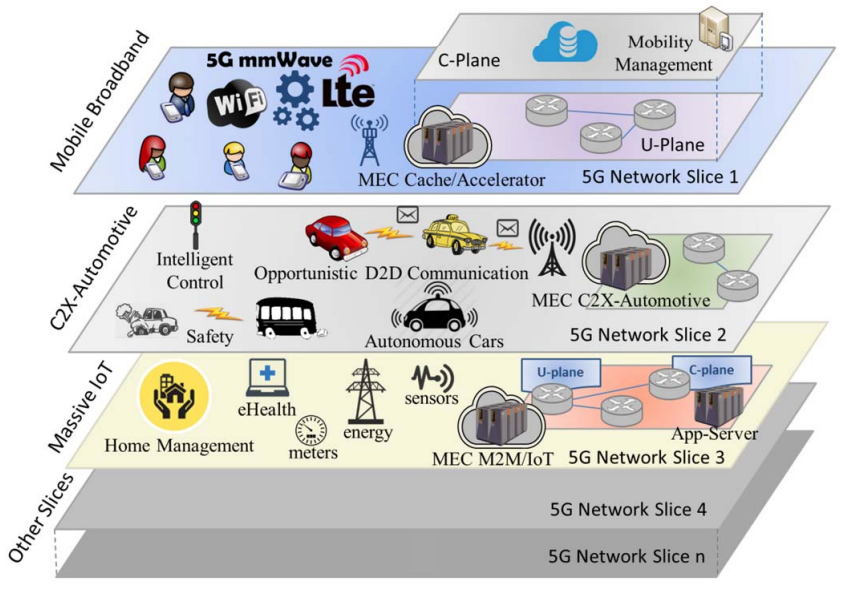
\includegraphics[width=\linewidth]{slice.png}
  \caption{Visualization of network slicing \cite{ref6_1}}
\end{figure}

\subsubsection{MEC Advantages} MEC, also known as multi-access edge computing, is an architecture standard from the European Telecommunications Standards Institute (ETSI) that attempts to shift the geographical location of where data processing occurs to be closer to end-users and their devices. This allows for faster data transmission and reduces the reliance on more distant core networks. The result is ultra-low latency via locally processed data, allowing for useful applications like autonomous driving, augmented reality, and smart city services. \cite{ref6_1} MEC also makes use of the extensive coverage of cellular networks to support machine-to-machine (M2M) communication and general Internet of Things (IoT) applications. MEC, albeit controversially, provides contextual data on user location, preferences, and interests which enables service providers to deliver more personalized experiences \cite{ref6_1}.
\begin{figure}[h]
  \centering
  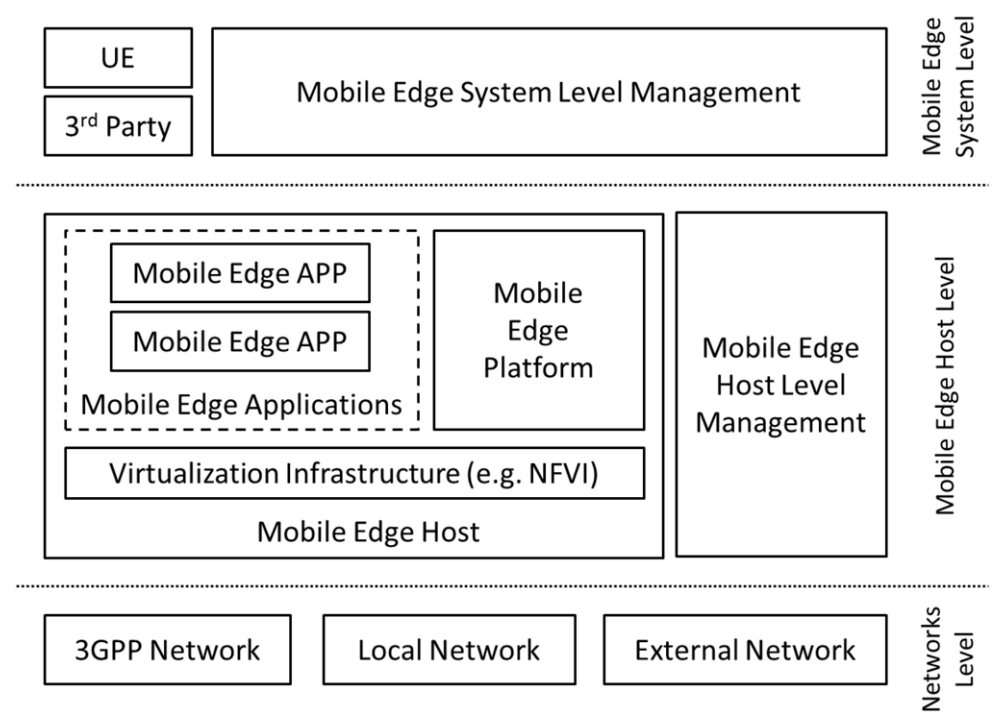
\includegraphics[width=\linewidth]{mec.png}
  \caption{ETSI MEC framework \cite{ref6_1}}
\end{figure}

\subsection{Vulnerabilities Introduced by 5G Advantages}
Although 5G’s use of advanced technologies offers notable benefits, they also create vulnerabilities that expand the attack surface. The following subsections analyze these vulnerabilities and emphasize their flaws.

\subsubsection{SDN Security Challenges}
SDN’s use of a logically centralized controller in the control plane can be a great attack vector due to the device being a single point of failure. All the flow requests, as well as the management and control of data packets, are processed by this centralized controller which makes it an obvious target for attackers. A successful attack on the SDN controller would mean the whole network could be controlled by a bad actor. This would mean the attacker could compromise sensitive information and disrupt entire network operations \cite{ref6}. \cite{Lee05}

A common type of attack that exploits this kind of vulnerability is the distributed denial-of-service (DDoS) attack. Attackers would flood the controller and overwhelm it with a high volume of traffic or control requests. This would exhaust the controller's resources which would primarily disrupt service availability. Smart devices like electricity meters could lose connection to electricity services. This would imply power outages and unstable connections for customers of MNOs and a loss of confidence in these MNOs \cite{ref3}.

\subsubsection{NFV Security Challenges}
NFV relies on a diverse set of hardware providers, virtualization platforms, and VNF developers. This diversity increases the potential weak spots of a network using NFV due to the shared nature of the various components. Each of these components, ranging from physical hardware to virtualized software layers, introduce unique risks. The complexity of managing them all creates opportunities for attackers to exploit misconfigurations and vulnerabilities. 

Hypervisors are essential in running virtualized software and play a critical role in NFV environments. If they are not properly maintained, they can be significant sources of vulnerabilities and potentially allow attackers to compromise VMs and gain unauthorized access to network resources. Attackers can exploit rapid reconfiguration and improperly isolated VNFs to bypass defenses or move through the system and disrupt critical network functions \cite{ref3_1}.

\subsubsection{Network Slicing Vulnerabilities}
The sharing of an infrastructure to create multiple shared networks introduces various security risks related to shared components. Misconfigurations in slice isolation can lead to cross-slice attacks, where a compromised slice can create severe consequences for other slices. Examples include unauthorized access to systems, DoS attacks on neighboring slices, and impersonation attacks. Side-channel attacks are another type of vulnerability that exploit the shared hardware and can result in exposing sensitive data across slices \cite{ref3_2}. The complexity of managing multiple slices increases the likelihood of configuration errors which increases the previously mentioned risks.

 The logical nature of network slices introduces risks in controlling communications across slices. Unprotected or poorly implemented inter-slice user-plane, signaling, or management-plane communications could be disrupted. This would allow attackers to interfere with the services provided by network slices or even initiate unauthorized interactions \cite{ref3_2}. 

Impersonation attacks pose a significant threat, particularly targeting network slice managers or host platforms. A bad actor could impersonate a network slice manager to deploy unauthorized slice instances on physical hosts, or a compromised host platform could falsely present itself as authorized. The potential implications of this are corruption, disclosure, or interruption of services for users \cite{ref3_2}.

\subsubsection{MEC Security Challenges}
The use of a distributed architecture in MEC creates notable security challenges that necessarily complicate security management. The avoidance of going through core networks and the involvement of third-party applications lead to potential billing risks and fraud. Valuable data is transmitted between users and the network edge, meaning the core networks are putting their trust in edge components to handle the sending of users' confidential records, like billing charges, to the home network. Edges of networks are more vulnerable to attack than core networks which creates a large risk of billing errors and fraud. Moreover, edge nodes in networks usually have a lot less computational power and make them great targets for DoS attacks. This can impact the network drastically and spoil the potential of ultra-low latency by degrading it to an unusable state \cite{ref3_3}. 

MEC often hosts third-party applications on the same platforms as critical network functions. If these applications are poorly designed or malicious, they can exhaust resources needed by network functions or introduce malware. This could lead to the compromise of the entire platform. In addition, applications have the ability to influence the configuration of the radio access network (RAN), resulting in the DoS of other users \cite{ref3_3}.

\bibliographystyle{ACM-Reference-Format}
\bibliography{main}

\end{document}
\endinput
%%
%% End of file `sample-acmtog.tex'.
